%% This is an example first chapter.  You should put chapter/appendix that you
%% write into a separate file, and add a line \include{yourfilename} to
%% main.tex, where `yourfilename.tex' is the name of the chapter/appendix file.
%% You can process specific files by typing their names in at the 
%% \files=
%% prompt when you run the file main.tex through LaTeX.
\chapter{Introduction}
\section{The Beginning}
\label{sec:vision}
  InMind began as an application designed to help bereaved individuals deal with
  some of their specific needs, specifically story, affect, and availability sharing.

  My initial prototype, InMourning, targeted three needs that became apparent
  from needfinding studies conducted by Massimi and
  Baecker \cite{mm11a, mm10, mm13},

  \begin{enumerate}
  \item \textbf{Affect Sharing} - The well being of bereaved individuals is often a subject
    of inquiry, and sharing this information is a common task.
  \item \textbf{Availability Sharing} -
    Caring friends and family often want to be present
    and available for the bereaved, however,
    the bereaved generally want to control the nature and timing of communication between
    them and their family, friends, and other supporters.
    The bereaved are sensitive to what kind
    of interaction (texts, calls, face-to-face visits) and when they occur (exactly
    what hour of what day, or frequency). The influx of media and ways to
    communicate actually make it consistently overwhelming for the bereaved,
    particularly added to the already stressful interactions that necessarily
    follow a loved one's passing.
    Thus, the availability of the bereaved, how able and willing they are
    to accommodate guests, is important to communicate.
  \item \textbf{Story Sharing} - Bereaved individuals feel a need to share stories related to
    or inspired by their relationship with the departed.
    From reflecting on a trigger, pattern, or thought that carries unusual
    significance for the mourner to full blown story telling, bereaved individuals
    consistently want to share aspects of their experience with caring friends and
    family, many of whom are likely mourning the same loss.
  \end{enumerate}

  These three needs were collected because they addressed the common theme of improving
  relationships with caring friends and family during the time of difficulty.

  In the context of these needs, I developed InMourning to work in an HCI study,
  in the theme of existing bereavement technologies,
  hoping to better understand how people can use technology to meet their needs.
  The initial prototypes of InMourning are attached to this in Appendix C.

  \subsection{Bereavement Technologies}
    For inspiration and guidance, I looked into existing bereavement technologies.
    Research into bereavement from the perspective of HCI is young, but the
    existing literature reveals some of the core problems that technology can
    address. Among the earliest research is that of Massimi and Baecker in 2010
    \cite{mm10},
    a needs-analysis of all the ways that technology intersects with the lives of
    the bereaved.
    Part of their study was an observation of how,
    in the potentially-dispersed setting of the modern world, 
    technology is already used to help bring people together during mourning.
    Massimi and Baecker proposed a wide set of design opportunities and challenges.
    They were primarily interested in exploring technological artifacts,
    both inherited from the deceased and those created by the bereaved to
    remember and grieve, but they also mention the possibility of technology
    helping to provide social support.

  % Homescreen Figure
  \begin{figure}
  \caption{\textbf{Besupp Screenshot} --
  Besupp offered circles for people with like losses to share thoughts
  and feelings with each other.
  }
  \centering
  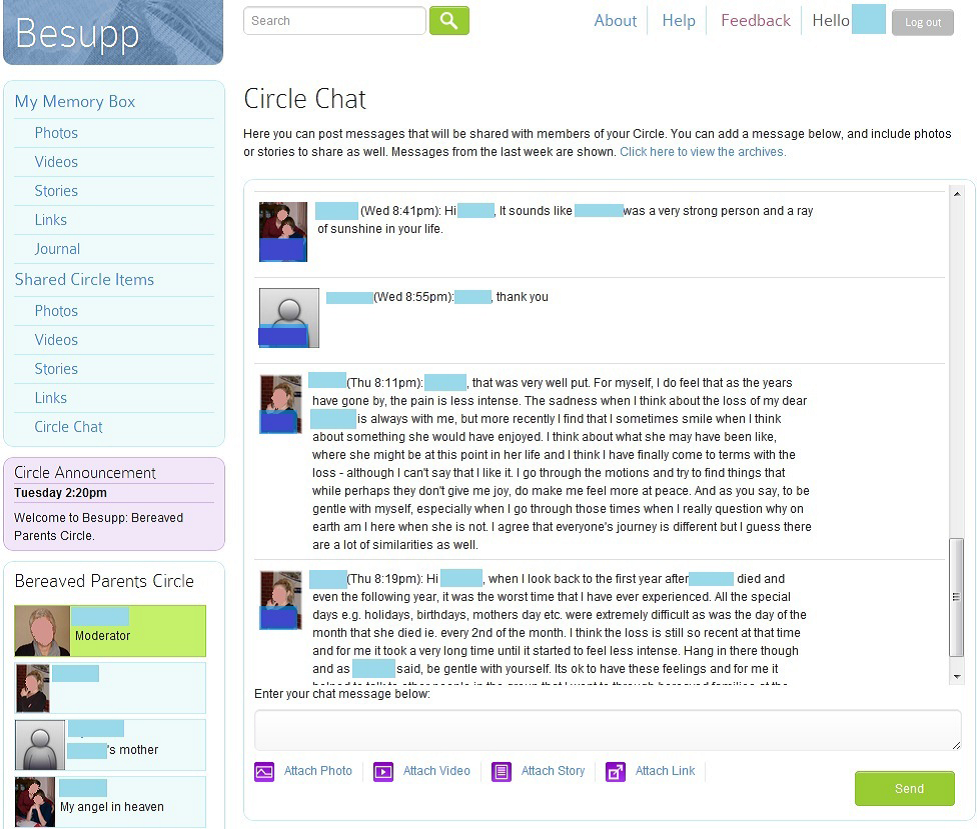
\includegraphics[width=0.65\textwidth]{besupp.png}
  \label{fig:besupp}
  \end{figure}

    There have been few technologies designed explicitly for the grieving. One
    example is Besupp, an online platform for maintaining a support group between
    people who have experienced similar losses, designed and tested by Massimi and
    co. in 2013. \cite{mm13}
    A screenshot from the study is shown in Figure \ref{fig:besupp}.
    Massimi and co. observed that technologies can be helpful as
    one of many ways to help with coping, as the needs of the bereaved are best
    addressed by a variety of interactions.
    This further study demonstrated that
    there is value in support systems that are maintained over long periods and
    designed for to low and intermittent usage.

    Other research has generally been observational, for instance Brubaker's study
    in 2011 of usage of existing technologies. \cite{brubaker11}

  \subsection{Maturation into InMind}
    However, we soon ran into a problem.
    If we want to use technology to improve the relationships between friends and family during the
    process of bereavement, we have to introduce technology well before the crisis happens.
    This is for primarily two reasons.
    \begin{enumerate}
    \item Death is often a stunning, overwhelming catastrophe,
    and bereaved individuals cannot be burdened with learning how to use a new technology.
    Many recently bereaved individuals already find it difficult to do things they normally can. \cite{??}
    \item For the deaths that are more forseeable, such as due to illness,
    there is often a long period of handling the dire situation,
    in which many of the same needs exist.
    In fact, mourning can sometimes begin before the death. \cite{??}
    \end{enumerate}

    Then, the more we explored the needs of bereaved individuals,
    and how to best reach out to them, the more we realized that these needs exist in some form
    for all people who are dealing with the difficult periods of life.
    Problems such as chronic illness, physical or psychological,
    can make the wellness, availability, and story of individuals relevant to those
    close to them.

